\documentclass[12pt,a4paper]{article}

% ---------------------------------------------------------------------------
% Relatório técnico — Fraudes PIX contestadas via MED (dados abertos do BCB)
% Compilação: tectonic relatorio.tex   (ou pdflatex, 2 passadas)
% ---------------------------------------------------------------------------
\usepackage[brazil]{babel}
\usepackage[T1]{fontenc}
\usepackage[utf8]{inputenc}
\usepackage{lmodern}
\usepackage[margin=2.5cm]{geometry}
\usepackage{graphicx}
\usepackage{booktabs}
\usepackage{microtype}
\usepackage{float}
\usepackage[hidelinks]{hyperref}
\usepackage{caption}
\captionsetup{font=small,labelfont=bf}

\graphicspath{{../notebooks/figuras/}}

\newcommand{\code}[1]{\texttt{#1}}

\title{\textbf{Fraudes no PIX via Mecanismo Especial de
Devolução:}\\ modelagem relacional, pipeline de ingestão e análise dos
dados abertos do Banco Central}
\author{Eduardo Carvalho Biagini de Mello
   \and Laura Nascimento Silva
   \and Jefferson Pereira de Souza
   \and Bruno Lima Soares}
\date{Junho de 2026}

\begin{document}

\maketitle

\begin{abstract}
\noindent Nesse trabalho, documentamos a construção de um projeto analítico que olha para as transações PIX contestadas por suspeita de fraude, no âmbito do Mecanismo Especial de Devolução (MED), a partir dos dados abertos publicados pelo Banco Central do Brasil. Atuamos da investigação das fontes e do desenho de um modelo relacional normalizado na terceira forma normal, na implementação física em PostgreSQL, desenvolvimento de um fluxo de ingestão e análise dos dados obtidos, chegando em cinco achados relevantes sobre o comportamento da fraude no arranjo PIX entre 2022 e 2026.
\end{abstract}

\section{Introdução}

O PIX transformou, em poucos anos, a forma como o brasileiro movimenta
dinheiro. No mesmo passo em que a agilidade permitiu rápida difusão do mecanismo, abriu brecha para golpes: uma transferência fraudulenta se completa em
segundos, e o dinheiro pode ser pulverizado em dezenas de contas antes que a
vítima sequer perceba o ocorrido. Como resposta, o Banco Central instituiu o
Mecanismo Especial de Devolução (MED), um rito formal pelo qual o usuário
pagador contesta uma transação sob suspeita de fraude e as instituições
envolvidas bloqueiam e, quando possível, devolvem os recursos.

Nosso projeto nasce da provocação: \emph{o que os dados públicos do
MED nos contam sobre a fraude no PIX?} Para responder com rigor, evitamos o
caminho do script descartável sobre um CSV e construímos a infraestrutura
completa: um modelo de dados relacional projetado com justificativa para cada
decisão, um banco PostgreSQL com restrições de integridade que protegem a
semântica do domínio, um pipeline de ingestão reprodutível e uma camada de
acesso que isola a análise dos detalhes do banco. O resultado é um conjunto
de análises que se sustenta sobre dados auditáveis, e uma base que pode ser
estendida para novas perguntas.

\section{Contexto do trabalho}

O trabalho foi desenvolvido como projeto prático da disciplina de Introdução
a Bancos de Dados, com um escopo deliberadamente profissional: tudo o que
fosse construído deveria se parecer com o que se espera de um time de dados
em produção. Isso se traduziu em quatro compromissos assumidos desde o
início.
\begin{itemize}
    \item Primeiro, modularidade: o código foi separado em camadas com responsabilidades claras (extração, transformação, carga, acesso e análise), em vez de um único script monolítico.
    \item Segundo, o acesso ao banco acontece exclusivamente por meio de um \emph{Data Accessor} (padrão DAO), de modo que nenhuma consulta SQL vaza para o código de análise. 
    \item Terceiro, reprodutibilidade: o projeto declara suas dependências, lê credenciais de variáveis de ambiente e pode ser recriado do zero com três comandos.
    \item Quarto, fidelidade aos dados reais: todas as etapas foram validadas com a API oficial do Banco Central e um banco PostgreSQL de verdade (para testes, um servidor local e, na versão final, uma instância gerenciada no Supabase).
\end{itemize}

O domínio analítico contempla quatro perspectivas: as
\emph{ocorrências de fraude} consolidadas pelo MED, as \emph{instituições
financeiras} participantes do arranjo, a \emph{dimensão geográfica}
(região, estado e município) e o \emph{período de tempo}, que passa por todas
as demais.

\section{Como os dados foram obtidos}

\subsection{As fontes}

O Banco Central publica os dados do PIX na plataforma Olinda, um serviço
OData de dados abertos. Antes de qualquer modelagem, inspecionamos o
catálogo de metadados do serviço (\code{\$metadata}) e coletamos amostras
reais de cada conjunto. Três fontes sustentam o projeto, todas com
competência mensal:

\begin{table}[H]
\centering\small
\begin{tabular}{lll}
\toprule
\textbf{Endpoint} & \textbf{Conteúdo} & \textbf{Granularidade} \\
\midrule
\code{EstatisticasFraudesPix} & contestações, devoluções e bloqueios do MED & nacional \\
\code{ChavesPix} & base de chaves por instituição (ISPB) & instituição \\
\code{TransacoesPixPorMunicipio} & volumetria transacionada & município \\
\bottomrule
\end{tabular}
\caption{Fontes de dados consumidas da API Olinda/BCB.}
\end{table}

Essa análise inicial revelou um aspecto que moldou todo o desenho analítico: o
conjunto de fraudes do MED é divulgado \emph{agregado nacionalmente}, sem
abertura por instituição ou por região. Optamos então por um novo caminho, abordando as dimensões de instituição e de geografia no modelo por meio das outras duas fontes,
e as análises que as utilizam tratam volumetria e crescimento de base de
chaves como \emph{variáveis de contexto e proxies de exposição ao risco},
nunca como medida direta de fraude por participante.

\subsection{As peculiaridades da API}

A integração com a API foi um dos desafios que enfrentamos, e julgamos
importante documentar o que encontramos, pois vai economizar tempo de quem
reutilizar esse trabalho. 

Os endpoints do serviço são \emph{function imports} OData que exigem um parâmetro de função na URL, por exemplo, \code{ChavesPix(Data=@Data)?@Data='2024-12-31'}, mas o servidor \emph{ignora o valor do parâmetro} e devolve a tabela inteira; o recorte efetivo precisa ser feito com a cláusula \code{\$filter}, que felizmente é aplicada no servidor. 

Descobrimos ainda que o parâmetro de paginação \code{\$skip=0} provoca um erro HTTP~500 (ele só pode ser enviado a partir da segunda página) e que o servidor rejeita espaços codificados como
\code{+} na query string, aceitando apenas \code{\%20}, o que nos obrigou a montar as URLs manualmente em vez de delegar a codificação à biblioteca HTTP. O cliente de extração resultante pagina os resultados, aplica \emph{retry} com recuo exponencial e registra em log cada lote extraído.

\section{O racional por trás da modelagem}

\subsection{Dimensões: tempo, geografia e instituições}

A primeira decisão estrutural foi organizar o modelo em torno de dimensões
compartilhadas. A dimensão \code{periodo} usa uma chave substituta
(\emph{surrogate key}) com unicidade garantida sobre o par (ano, mês). Adicionamos uma coluna de data materializada pelo próprio SGBD (\code{GENERATED ALWAYS AS make\_date(ano, mes, 1) STORED}), que oferece a conveniência de filtros por intervalo de datas sem risco de divergir dos campos que a originam. O banco, e não a aplicação, é o responsável pela coerência.

Para a geografia e as instituições, fizemos a escolha oposta: chaves
\emph{naturais}. Municípios e estados já possuem códigos IBGE estáveis e
universais, e as instituições financeiras são identificadas pelo ISPB, um
código público de oito dígitos. Adotar esses identificadores como chave
primária elimina uma camada de tradução e torna o banco diretamente
comparável a qualquer outra base que use as mesmas convenções. A hierarquia
geográfica foi decomposta em três tabelas encadeadas
(\code{regiao} $\rightarrow$ \code{estado} $\rightarrow$ \code{municipio}),
e o seed das duas primeiras, domínios estáveis do IBGE, foi embutido no
próprio DDL, de modo que o pipeline de ingestão só precisa carregar dados
dinâmicos.

\subsection{Lidando com o volume dos dados}

O registro mensal do MED chega da API como uma linha com 24 colunas que
misturam assuntos: contestações, devoluções integrais e parciais, três
motivos de não devolução e dois desfechos de bloqueio cautelar. Espelhar
esse formato no banco seria cômodo, mas perpetuaria grupos repetitivos
(pares quantidade/valor para cada categoria) e tornaria qualquer agregação
por categoria uma ginástica de \code{CASE WHEN}. Em vez disso, o registro
foi decomposto em um fato principal (\code{fraude\_med}, uma linha por mês)
e três tabelas de detalhamento (\code{devolucao\_med},
\code{nao\_devolucao\_med}, \code{bloqueio\_cautelar}) em que a categoria, tipo de devolução, motivo da falha, desfecho do bloqueio, é um
atributo discriminador que compõe a chave primária. O mesmo princípio guiou
o fato municipal: as doze colunas de medida (valor, quantidade e pessoas
para cada combinação de pagador/recebedor com PF/PJ) viraram uma linha por
combinação, com papel e natureza como colunas categóricas.

\subsection{Integridade declarativa como linha de defesa}

Uma convicção atravessa o projeto físico: restrição que pode ser declarada
no banco não deve ser responsabilidade da aplicação. Os domínios categóricos
fechados viraram tipos \code{ENUM} nativos do PostgreSQL, é impossível
inserir um motivo de não devolução fora do vocabulário do MED. Valores
monetários usam \code{NUMERIC(18,2)} (jamais ponto flutuante), contagens
usam \code{BIGINT} com \code{CHECK} de não negatividade, e o ISPB é texto
com verificação de formato por expressão regular, preservando zeros à
esquerda. Duas restrições merecem destaque por codificarem semântica de
negócio: a soma de contestações aceitas e rejeitadas não pode exceder o
total contestado no mês, e os dois primeiros dígitos do código IBGE de um
município devem coincidir com o código do estado ao qual ele declara
pertencer. Essa última pegou, durante os testes, exatamente o tipo de
inconsistência que dados públicos costumam carregar.

\section{As três etapas da normalização}

Vale percorrer as três formas e o que cada uma exigiu deste domínio em particular.

\paragraph{Primeira forma normal.} A 1FN exige atributos atômicos e a
ausência de grupos repetitivos. O inimigo aqui era o formato de publicação
do BCB: colunas como ``valor devolvido integralmente'' e ``valor devolvido
parcialmente'' são, na essência, o mesmo atributo (valor devolvido)
qualificado por uma categoria implícita no nome da coluna. Nossa estratégia
foi identificar cada família de colunas que variava apenas pela
categoria embutida no nome e convertê-la em linhas, materializando a
categoria como coluna discriminadora. Foi assim que 24 colunas do registro
de fraude se tornaram quatro tabelas estreitas, e doze colunas do registro
municipal se tornaram quatro linhas por município.

\paragraph{Segunda forma normal.} A 2FN elimina dependências parciais:
nenhum atributo não chave pode depender de apenas parte de uma chave
composta. Como a decomposição da 1FN produziu várias tabelas de chave
composta, verificamos cada uma delas. Em \code{transacao\_municipio}, cuja
chave é (período, município, papel, natureza), as medidas de valor e
quantidade dependem da combinação completa, não existe ``valor do
município'' sem especificar o mês, o papel e a natureza. O risco clássico de
violação seria armazenar ali o nome do município, que depende só do código
IBGE: esse atributo foi mantido exclusivamente na tabela \code{municipio}.
O mesmo raciocínio levou o nome da instituição para fora do fato de chaves
PIX, cuja chave composta inclui o ISPB.

\paragraph{Terceira forma normal.} A 3FN remove dependências transitivas:
atributos não chave que dependem de outros atributos não chave. O caso mais
ilustrativo do domínio é a geografia. No CSV de origem, cada linha municipal
repete o nome do estado, a sigla e o nome da região, todos
transitivamente dependentes do código do município. Na nossa decomposição,
o município conhece apenas o seu estado, e o estado conhece apenas a sua
região. Sigla e nome de região existem uma única vez no banco. Tomamos uma
decisão sobre métricas derivadas publicadas pelo BCB (como o
percentual de devolução): elas foram \emph{mantidas} no fato mensal, por
fidelidade ao dado oficial, recalcular a partir das demais colunas
poderia introduzir divergências de arredondamento em relação ao que o
regulador divulga, e o custo em redundância é de uma coluna por mês.

\section{Insights obtidos}

A análise exploratória consumiu exclusivamente a camada de acesso a dados,
que encapsula as consultas SQL, de projeções simples a uma consulta
analítica com funções de janela (\code{LAG} e \code{RANK} particionados),
e devolve \emph{DataFrames} prontos para visualização. Cinco achados
merecem registro.

\subsection{A ruptura de regime no fim de 2025}

\begin{figure}[H]
\centering
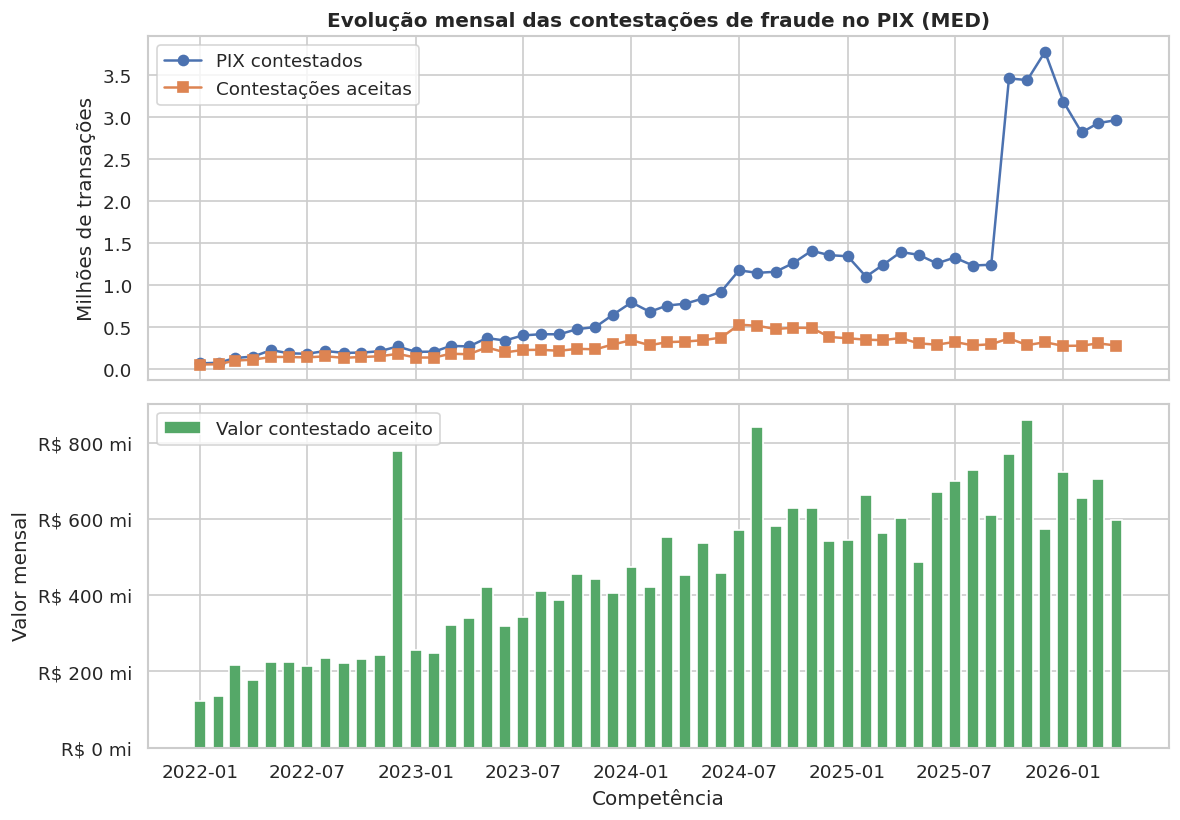
\includegraphics[width=0.92\textwidth]{01_evolucao_contestacoes.png}
\caption{Evolução mensal das contestações de fraude no PIX (MED).}
\end{figure}

Foram 53,0 milhões de PIX contestados no período (jan/2022 a abr/2026), com
R\$~24,52 bilhões reconhecidos como fraude. O padrão dominante do gráfico é o
salto de outubro de 2025: o volume mensal de contestações sobe de cerca de
1,2 milhão para 3,5 milhões (+178\%), mas as contestações \emph{aceitas} permanecem
estáveis em torno de 350 mil mensais. A leitura crítica é que o salto não
sinaliza uma explosão de fraude consumada, e sim a facilitação do canal de
contestação: quando contestar fica mais fácil, contesta-se mais, inclusive o
que não se confirma. A taxa de aceite despenca de cerca de 40\% para 10\%,
e o custo operacional de triagem das instituições cresce sem contrapartida
de fraude real.

\subsection{A fraude cresce mais rápido que o próprio PIX}

\begin{figure}[H]
\centering
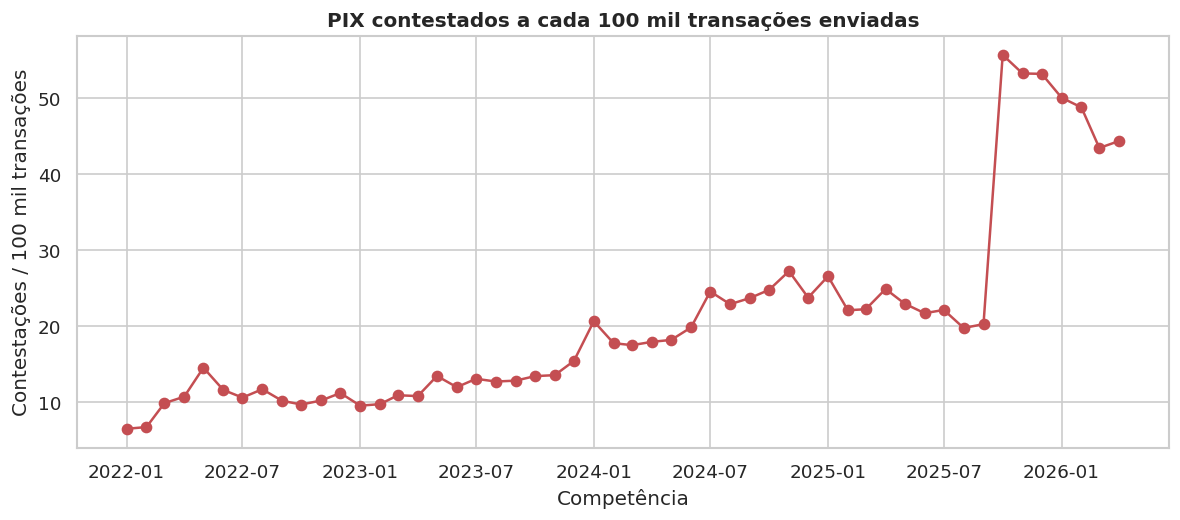
\includegraphics[width=0.92\textwidth]{02_taxa_contestacao.png}
\caption{PIX contestados a cada 100 mil transações enviadas.}
\end{figure}

Para separar o crescimento da fraude do crescimento do sistema,
normalizamos as contestações pelo volume nacional de transações (obtido por
subconsulta sobre o recorte municipal). A taxa parte de 6,5 contestações
por 100 mil transações no início de 2022, atinge o pico de 55,7 e recua
para 44,4 ao fim da série (abr/2026). Mesmo descontado o uso crescente do
PIX, a propensão a contestar mais que sextuplicou ao longo do período, um argumento direto para
investimento em prevenção, e não apenas em remediação.

\subsection{O dinheiro some antes de o MED alcançar}

\begin{figure}[H]
\centering
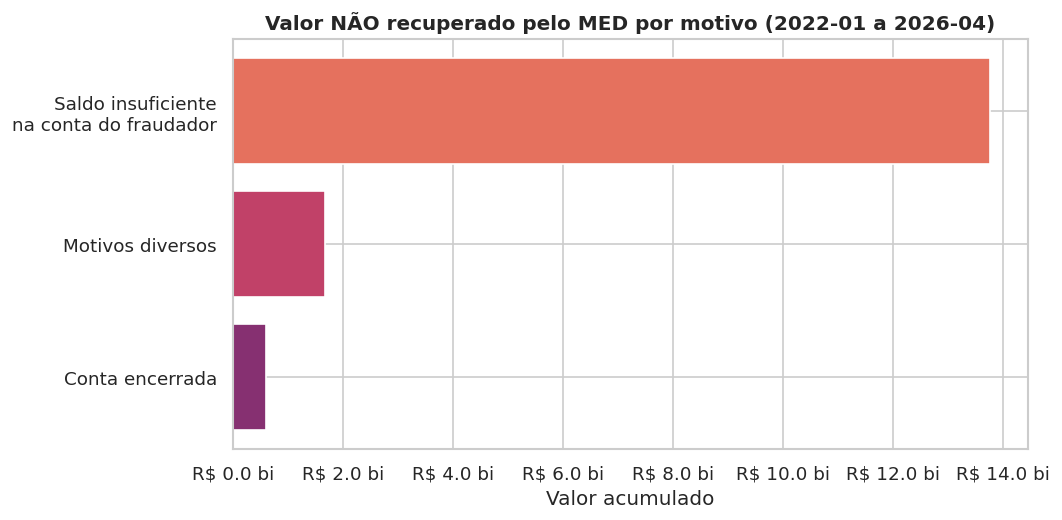
\includegraphics[width=0.88\textwidth]{03_funil_nao_devolucao.png}
\caption{Valor não recuperado pelo MED, por motivo (2022--2026).}
\end{figure}

Dos valores aceitos como fraude, R\$~16,04 bilhões não retornaram às vítimas
no período, e 85,8\% desse total falha por um único motivo: saldo
insuficiente na conta do fraudador. Conta encerrada e motivos diversos são
marginais. O insight operacional é claro: o fraudador pulveriza
ou saca os recursos em minutos, antes que a contestação seja processada. A
janela de recuperação, e não a qualidade da análise, é o fator crítico do
mecanismo, o que explica e justifica a aposta regulatória nos bloqueios
cautelares.

\subsection{Concentração geográfica do fluxo}

\begin{figure}[H]
\centering
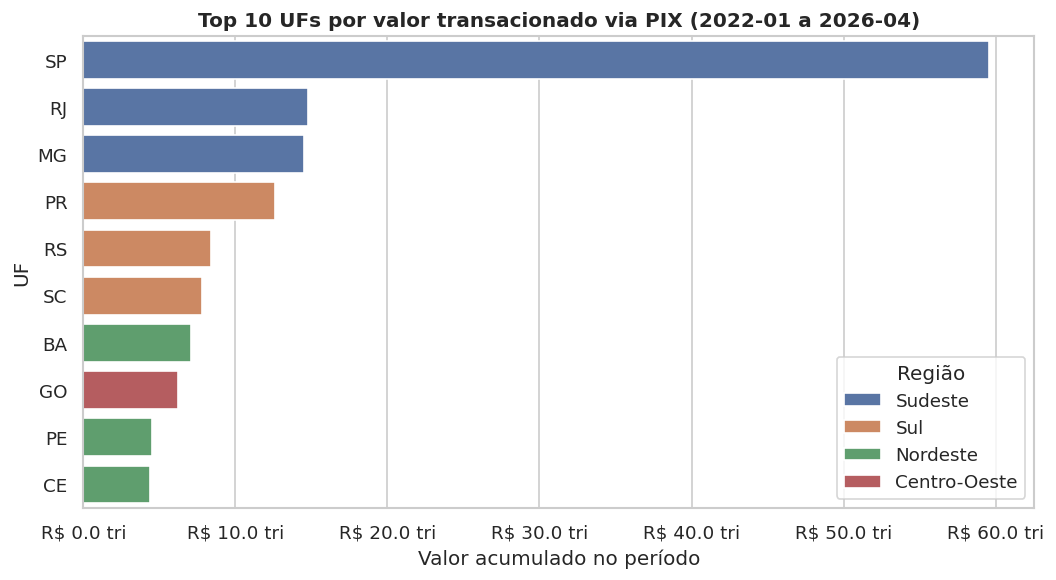
\includegraphics[width=0.88\textwidth]{04_volume_por_uf.png}
\caption{Dez maiores UFs por valor transacionado via PIX no período (2022--2026).}
\end{figure}

Três unidades federativas, São Paulo, Rio de Janeiro e Minas Gerais,
concentram 51,3\% de todo o valor transacionado no período. A consulta com
agregações e corte por \code{HAVING} revela ainda a assimetria interna:
Minas lidera em municípios ativos (853) movimentando um quarto do valor de
São Paulo, retrato de um interior pulverizado contra uma capital
concentrada. Para gestão de risco, a concentração indica onde o
monitoramento tem maior alavancagem absoluta.

\subsection{O outlier que valida o método}

\begin{figure}[H]
\centering
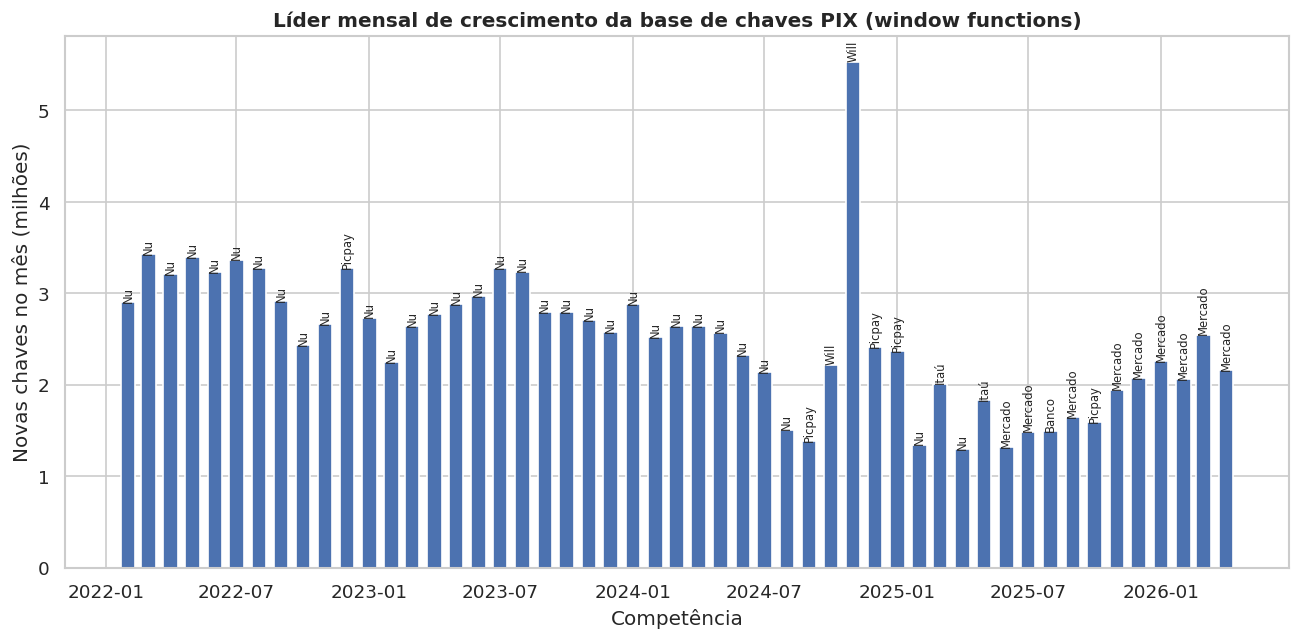
\includegraphics[width=0.95\textwidth]{05_ranking_crescimento_chaves.png}
\caption{Líder mensal de crescimento da base de chaves PIX.}
\end{figure}

A consulta analítica com funções de janela revela a disputa mensal pela
expansão de base de chaves: Nubank domina 2024, PicPay e Itaú alternam-se no
início de 2025 e o Mercado Pago assume o fim do período, com incrementos
mensais de 1,3 a 2,6 milhões de chaves. O achado mais valioso, porém, é o
ponto fora da curva: a Will Financeira, formalmente ``em liquidação
extrajudicial'', cresceu +246.356\% em outubro de 2024, saltando de
poucos milhares para 5,5 milhões de chaves em dois meses. Crescimento
explosivo de base em uma instituição em situação cadastral anômala é
exatamente o tipo de sinal que um monitoramento construído sobre este
modelo de dados levantaria para investigação humana, e valida o uso do
crescimento de chaves como proxy de exposição ao risco no arranjo.

\section{Conclusão}

O projeto cumpriu o ciclo completo que se propôs: da investigação das
fontes à análise final, passando por modelagem, infraestrutura física e
pipeline de ingestão. Algumas lições se destacam. A primeira é que a
qualidade da análise começa muito antes do gráfico: foi a inspeção
dos metadados da API que revelou a granularidade real do dataset
de fraudes e impediu que o projeto prometesse análises que os dados não
sustentam. A segunda é que normalizar não é burocracia: a decomposição em
3FN converteu um CSV hostil em tabelas que respondem perguntas de negócio
com SQL direto e legível. A terceira é o valor da integridade declarativa:
delegar ao SGBD a defesa da semântica do domínio (enums, checks,
hierarquias) tornou o pipeline mais simples e pegou inconsistências reais
dos dados públicos durante a carga.

Os números, por fim, contam uma história que merece atenção de quem opera e
regula o arranjo: a contestação cresce mais rápido que o sistema, a
recuperação esbarra na velocidade do fraudador, e os sinais mais
interessantes muitas vezes estão nos outliers estruturais, não nas
médias. Como trabalhos futuros, a base comporta naturalmente a incorporação
de novas competências (o pipeline é idempotente), o cruzamento com outros
conjuntos do BCB e a construção de alertas automatizados sobre os padrões
de crescimento anômalo que este estudo identificou manualmente.

\end{document}